\section{Поверхности}

\subsection{Двулучевая функция отражательной способности (ДФОС)}

Очевидно, что яркость точки на поверхности как-то зависит от материала поверхности,
на которую падает свет. Иначе говоря, яркость зависит от так называемых отражательных
способностей поверхности. На Рис. \eqref{brdf} компьютером отрисованы различные сферы.
В данном примере и камера и источник света находятся относительно далеко от сфер.
Причина, по которой мы видим их различными -- их материал, или различные отражательные способности.

\begin{figure}[h]
  \centering
  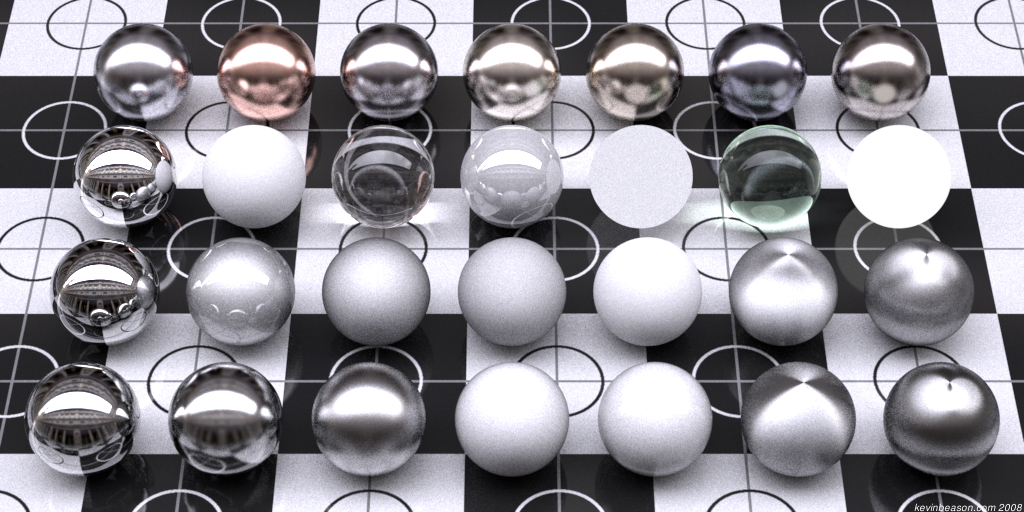
\includegraphics[scale=0.3]{tex/brdf.png}
  \caption{Пример разных отражательных способностей}
  \label{brdf}
\end{figure}

Возникает идея формализировать представление отражательных способностей любого материала,
с чем нам поможет двулучевая функция отражательной способности или ДФОС.

Для определения нам важны направления: направление света, падающего на предмет, и направление
отраженного и полученного света. Двулучевая функция, потому что речь будет идти про два луча.

\begin{figure}[h]
  \begin{center}
    \begin{tikzpicture}
      \def\SndrColor {yellow};
      \path (-5,4) pic [rotate=320,transform shape] (Sndr) {lighter};
      \node[left,text width=2.5cm] at (Sndr-body.south east) {Источник (Прожектор)};

      \def\RcvrColor {gray};
      \path (5,4) pic [rotate=130,transform shape] (Rcvr) {camera};
      \node[right,text width=2.5cm] at (Rcvr-body.south west) {Получатель (Камера)};

      \node [draw,
        trapezium,
        shade,
        minimum width=3cm,
        trapezium left angle=120,
        trapezium right angle=60] (Srfc) at (0, 0){};

      \draw[-Stealth, thick]
      (Srfc.center) coordinate (beginN)
      -- ([shift={(0,1.5)}]Srfc.center) coordinate (endN) node[above]{$\norm$};

      \draw[-Stealth,color=\SndrColor,line width=0.5mm]
      (Sndr-head)
      --node[left,color=black]{$(\theta_i,\phi_i)$} (Srfc.center) coordinate (endSnd);

      \draw[-Stealth,color=\RcvrColor,line width=0.5mm]
      (Srfc.center) coordinate (beginRcv)
      --node[right,color=black]{$(\theta_r,\phi_r)$} (Rcvr-head);

    \end{tikzpicture}
    \caption{Отражение поверхности}
    \label{surface_reflection}
  \end{center}
\end{figure}

Таким образом, чтобы представить свойства отражения любого материала,
мы хотим иметь возможность описать его свойства как с точки зрения
направления освещения, так и с точки зрения направления взгляда или направления отражения.

Выражая направление источника в полярных координатах через углы $(\theta_i,\phi_i)$ и
направление отраженного света через $(\theta_r,\phi_r)$, мы можем следующее
\begin{enumerate}
  \item Освещенность поверхности зависит от углов $(\theta_i,\phi_i)$, то есть $E:=E(\theta_i,\phi_i)$.
  \item Яркость поверхности зависит от углов $(\theta_r,\phi_r)$, то есть $L:=L(\theta_r,\phi_r)$.
\end{enumerate}

И теперь мы можем описать отражательную способность как двулучевую функцию отражательной
способноси:
\begin{equation}
  \rho(\theta_i,\phi_i,\theta_r,\phi_r)=\frac{L(\theta_r,\phi_r)}{E(\theta_i,\phi_i)}
\end{equation}

Измеряется в ср$^{-1}$, где стерадиан (ср) - единица измерения телесного угла. Перечислим некоторые свойства ДФОС:
\begin{enumerate}
  \item Неотрицательность: $\rho(\theta_i,\phi_i,\theta_r,\phi_r)>0$. Следует из того, что и
        яркость, и освещенность неотрицательны, значит и их отношение.
  \item Удовлетворяет равенству Гельмгольца: $\rho(\theta_i,\phi_i,\theta_r,\phi_r)=\rho(\theta_r,\phi_r,\theta_i,\phi_i)$.
        Это нам говорит о том, что поменяв местами прожектор и камеру, мы получим то же самое значение ДФОС.
\end{enumerate}

Существуют множество поверхностей, которые отражают одинаковое количество света
вне зависимости от вращения этой поверхности вокруг ее нормали. Такие
поверхности называют \textit{изотропными}, в обратном случае \textit{анизотропными}.
Когда говорят об изотропных поверхностях ДФОС определяют как функцию принимающую три
аргумента вместо четырех: $\rho(\theta_i,\theta_r,\phi)$.

\subsection{Механизмы, порождающие отражение}

Давайте поговорим об основных механизмах, порождающие отражение света.

\begin{figure}[h]
  \centering
  \begin{minipage}{.5\textwidth}
    \centering
    \begin{tikzpicture}
      \node [draw,
        rectangle,
        minimum width=6cm,
        minimum height=0.5cm,
      ] (obj) at (0, -1){};

      \draw[-Stealth, thick, black] (-3,3) coordinate (src) --node[above, midway, sloped]{Источник} ($ (obj.north east)!.5!(obj.north west) $) coordinate (middle);
      \draw[-Stealth, thick, blue] (middle) --node[above, midway, sloped]{Зеркальное отражение} (3,3) coordinate;
    \end{tikzpicture}
  \end{minipage}%
  \begin{minipage}{.5\textwidth}
    \centering
    \begin{tikzpicture}
      \node [draw,
        rectangle,
        pattern=bricks,
        minimum width=6cm,
        minimum height=1cm,
      ] (obj) at (0, -1){};
      \draw[-Stealth, thick, black] (-3,3) coordinate (src) --node[above, midway, sloped]{Источник} ($ (obj.north east)!.5!(obj.north west) $) coordinate (middle);
      \node [circle,
        inner sep=0pt,
        outer sep=0pt,
        minimum size=3cm] (C1) at (0,1) {};
      \draw[-Stealth, thick, red] (middle) -- (C1.north) coordinate node[right]{Диффузное отражение};
      \draw[-Stealth, thick, red] (middle) -- (C1.north west) coordinate;
      \draw[-Stealth, thick, red] (middle) -- (C1.north east) coordinate;
      \draw[-Stealth, thick, red] (middle) -- (C1.west) coordinate;
      \draw[-Stealth, thick, red] (middle) -- (C1.east) coordinate;
      \draw[-Stealth, thick, red] (middle) -- (C1.south west) coordinate;
      \draw[-Stealth, thick, red] (middle) -- (C1.south east) coordinate;
      \node [circle,
        inner sep=0pt,
        outer sep=0pt,
        rotate=22.5,
        minimum size=3cm] (C2) at (0,1) {};
      \draw[-Stealth, thick, red] (middle) -- (C2.north) coordinate;
      \draw[-Stealth, thick, red] (middle) -- (C2.north west) coordinate;
      \draw[-Stealth, thick, red] (middle) -- (C2.north east) coordinate;
      \draw[-Stealth, thick, red] (middle) -- (C2.west) coordinate;
      \draw[-Stealth, thick, red] (middle) -- (C2.east) coordinate;
      \draw[-Stealth, thick, red] (middle) -- (C2.south) coordinate;
      \draw[-Stealth, thick, red] (middle) -- (C2.south west) coordinate;
      \draw[-Stealth, thick, red] (middle) -- (C2.south east) coordinate;
    \end{tikzpicture}
  \end{minipage}
  \caption{Диффузное и зеркальное отражение}
  \label{reflect}
\end{figure}

Рассмотрим рис. \eqref{reflect}. Различают три механизма:
\begin{itemize}
  \item Первый - отражательная способность поверхности. Свет падает на поверхность
        и отражение происходит на самой плоскости. Такое отражение света называется
        \textit{зеркальны м} отражением. Оно придает поверхностям глянцевый или блестящий
        вид и свойственно гладким однородным материалам (зеркалам, стеклу, полированным металлам).
  \item Второй случай возникает, когда часть света проходит сквозь поверхность
        и проникает внутрь материала. Обычно вещества неоднородны и содержат различные
        частицы с разными показателями преломления. В результате попадающий внутрь свет
        преломляется и отражается несколько раз, отскакивает внутри случайным образом.
        Это происходит на небольшой глубине под поверхностью, поэтому частицы света
        проникают обратно и рассеиваются во многих направлениях.
        Это явление называется \textit{диффузным}. Из-за неоднородности среды
        объекты обладают матовостью.
  \item При анализе яркости точки изображения надо учитывать, что это результат отражения света из окружающей среды, который имеет составляющие
        диффузного и поверхностного отражения. Чаще всего встречается \textit{гибридное} отражение — комбинация этих двух механизмов.
\end{itemize}

\subsection{Модели отражения}

Рассмотрим широко используемые модели отражения.

\subsubsection{Светорассеивающая поверхность, закон Ламберта}

Большинство предметов, с которыми нам чаще всего приходится работать в жизни
(бумага, песок, камень, мел), рассеивают падающий на них свет таким образом,
что их яркости в разных направлениях оказываются примерно одинаковыми.

В 1760 году немецкий ученый Ламберт сформулировал закон, согласно которому
\textit{яркости светорассеивающей поверхности во всех направлениях одинаковы}.
Хоть и установлено, что не существует предмета, который бы строго удовлетворял
закону Ламберта, этот закон часто используют в компьютерном зрении и
компьютерной графике, потому что несмотря на ее простоту она
позволяет достаточно точно описывать многие поверхности.

\begin{figure}[h]
  \centering
  \begin{tikzpicture}
    \draw [name path=arc] (0,0) arc (0:180:4cm and 4cm) -- cycle;
    \node [
      rectangle,
      name path=rec,
      minimum width=1cm,
      minimum height=0.2cm,
      pattern=north east lines] (rec) at (-4,-0.1){};
    \node [below] at (rec.south){$\sigma$};
    \path [name path=ll-rec] (-9,3.75) coordinate (ll) -- (rec.north) coordinate (m);
    \path [name path=lu-rec] (-8,4.25) coordinate (lu) -- (m);
    \path [name path=rl-rec] ( 1,3.75) coordinate (rl) -- (m);
    \path [name path=ru-rec] ( 0,4.25) coordinate (ru) -- (m);
    \path [name intersections={of=ll-rec and arc,by=A}];
    \path [name intersections={of=lu-rec and arc,by=B}];
    \path [name intersections={of=rl-rec and arc,by=C}];
    \path [name intersections={of=ru-rec and arc,by=D}];
    \fill [pink, opacity=0.3] (A) -- (C) -- (D) -- (B);

    \draw (A) -- (m) -- (C);
    \draw (B) -- (m) -- (D);
    \draw [dashed] (A) node [left] {$A$} -- (C) node [right] {$C$};
    \draw [dashed] (B) node [left] {$B$} -- (D) node [right] {$D$};
    \draw [->] let \p1 = (m) in (m) -- (\x1,4.2) coordinate (N) node[above]{$\norm$};
    \pic [<->, draw, angle radius=15mm,"$\phi$",angle eccentricity=1.2] {angle=D--m--N};
    \pic [<->, draw, angle radius=15mm,"$\d\phi$",angle eccentricity=1.2] {angle=C--m--D};
  \end{tikzpicture}
  \caption{Расчет светового потока, излучаемого поверхностью с постоянной яркостью}
  \label{lambert::pic}
\end{figure}

На Рис. \eqref{lambert::pic} рассматривается площадка площади $\sigma$,
яркость $L$ которой одинакова во всех направлениях.
Сила света в направлении к точке $D$: $I=L\sigma\cos\phi$.
Рассмотрим телесный угол $\d\omega$, заключенный между двумя конусами,
полученными вращениями прямых проведенных от середины
площадки до точек $C$ и $D$ вокруг нормали $\norm$. Посчитаем его значение:
$$\d\omega=2\pi(\cos\phi-\cos\phi\cos\d\phi+\sin\phi\sin\d\phi)\approx 2\pi\sin\phi\d\phi$$
Так как сила света внутри этого телесного угла постоянна, то световой поток, получаемый из площадки:
$$\d\Phi=I\d\omega=2\pi L\sigma\cos\phi\sin\phi\d\phi$$
Тогда чтобы получить световой поток, излучаемой площадкой, для всей полусферы:
\begin{equation}\label{lambert::eq}
  \Phi=2\pi L\sigma\int_0^{\frac{\pi}{2}} \cos\phi\sin\phi\d\phi=\pi L\sigma\sin^2\phi\vert_0^\frac{\pi}{2}=\pi L\sigma
\end{equation}
Если взять в качестве площадки объект, который отражает весь падающий на него поток
и рассеивает его так, что яркость во все стороны оказывается одинаковой (удовлетворяет свойствам
\textit{идеального рассеивателя}), то выражение \eqref{lambert::eq} можно
переписать следующим образом:
$$\frac{1}{\pi}=\frac{L\sigma}{\Phi}=\frac{L}{E}=\rho(\theta_i,\theta_r,\phi)$$
Получается, что для светорассеивающей поверхности, удовлетворяющей закону Ламберта, ДФОС
является константой.

Поверхность любого тела не обладает свойствами идеального рассеивателя,
поэтому для того чтобы численно характеризовать изменение яркости
в разных направлениях используют \textit{коэффициент диффузии} или \textit{альбедо}.
Принято обозначать греческой буквой $\beta$, $0\leq\beta\leq1$.
Тогда выражение ДФОС по фиксированному направлению для любого тела имеет вид:
\begin{equation}
  \rho(\theta_i,\phi_i,\theta_r,\phi_r)=\frac{\beta}{\pi}
\end{equation}

\subsubsection{Зеркальная поверхность}

Рассмотрим противоположную модель - модель для идеально зеркальной поверхности.
Все отражение происходит на поверхности, диффузное отражение отсутствует.
В этом случае вся энергия падающего света отражается в одном направлении.

\begin{figure}[h]
  \begin{center}
    \begin{tikzpicture}
      \def\SndrAngle {320};
      \def\SndrColor {yellow};
      \def\RcvrColor {gray};
      \path (-5,4) pic [rotate=\SndrAngle,transform shape] (Sndr) {lighter};
      \path (4.5, 2) pic [rotate=120,transform shape] (Rcvr) {camera};

      \node [draw,
        trapezium,
        shade,
        minimum width=3cm,
        trapezium left angle=120,
        trapezium right angle=60] (Srfc) at (0, 0){};

      \draw[-Stealth, thick]
      (Srfc.center) coordinate (beginN)
      -- ([shift={(0,1.5)}]Srfc.center) coordinate (endN) node[above]{$\norm$};

      \draw[-Stealth,color=\SndrColor,line width=0.5mm]
      (Sndr-head)
      --node[left,color=black]{$(\theta_i,\phi_i)$} (Srfc.center) coordinate (endSnd);

      \draw[-Stealth, dashed, color=blue, line width=0.5mm]
      let \p1=(Sndr-head) in
      (Srfc.center) --node[above, midway, sloped]{Зеркальное отражение} (-\x1,\y1);

      \draw[-Stealth,color=\RcvrColor,line width=0.5mm]
      (Srfc.center) coordinate (beginRcv)
      --node[right,color=black]{$(\theta_r,\phi_r)$} (Rcvr-head);

    \end{tikzpicture}
    \caption{Отражение зеркальной поверхности}
    \label{specular_surface}
  \end{center}
\end{figure}

ДФОС в случае идеального зеркала выглядит следующим образом:

\begin{equation}
  \rho(\theta_i,\phi_i,\theta_r,\phi_r)=\frac{\delta(\theta_i-\theta_r)\delta(\phi_i+\pi-\phi_r)}{\cos\theta_i\sin\theta_i}
\end{equation}

где $\delta(x)=\begin{cases}
    1, & x=0    \\
    0, & x\neq0
  \end{cases}$, то есть это обозначает, что наблюдатель видит свет только когда вектор наблюдения совпадает с вектором отражения.

В знаменателе произведение косинуса и синуса, коэффициент пропорциональности, обеспечивающий выполнение закона сохранения энергии: весь свет, отражаемый сферой независимо от направления, равен свету, падающему на поверхность.
